\section{Experiments and Results}\label{sec:experiments}
After presenting the separation constraints, we test our formulation in an set of experiments in order to show its validity.

We wish to find if using the separation constraints we can use deeper networks given the same width. Hereby, we train a set of networks following a grid of combinations of depth and width. We do not use an existing "production" architecture since they explicitly employ techniques which we wish to avoid (recall Table \ref{tab:techniquesTable}),  as we explained in the introduction \ref{sec:introduction}. We benchmark it to \ReLU and the most common instance of Data Normalization family, Batch Normalization \cite{batchnorm}, as baselines, against our three versions of the separation constraints: unit separation (\SepUnit), point separation (\SepPoint) and their combination (\SepUnitPoint). 
\\\\
We use three different datasets in our experimentation: the \moons dataset (sampling $100$ points, $85$ for training and $15$ for validation), the \texttt{MNIST} dataset \cite{mnist} and the \texttt{CIFAR-10} dataset \cite{cifar10}.
\\\\
We train a set of networks whose depth ranges from $1$ to $150$ layers deep and from $1$ to $25$ units wide, in the case of \moons, from $2$ to $64$ layers deep and from $2$ to $8$ units wide for \texttt{MNIST} and, from $2$ to $40$ layers deep and $10$ units wide for \texttt{CIFAR-10}. We optimize the networks using Adam \cite{adam}. We use a learning rate of $0.01$ for $10000$ epochs using a batch size of $85$ for \moons and learning rate of $0.001$ for $50$ epochs using a batch size of $1024$ for \texttt{MNIST} and \texttt{CIFAR-10}. As an initialization scheme we use Glorot uniform \cite{Glorot10Initialization} (used by default on \texttt{Keras}). We use a value of $\lambda$ of $10^-4$ for \moons and $10^{-8}$ for \texttt{MNIST} and \texttt{CIFAR-10} when needed. We fix the random seed to an arbitrary value of $10$. 
\\\\
We also wish to assess that our proposal is robust to stochasticity. We train a thin and deep network composed of 50 layers of 4 units each (i.e. $m_k=4$ for $k=1,\ldots,D$, which would be impossible to train without resorting to additional techniques (recall Table \ref{tab:techniquesTable}), using $10$ different random seeds. We use the \moons dataset as described earlier due computational constraints. We use a learning rate of $0.01$ for $10000$ epochs using a batch size of $85$. As an initialization scheme we use Glorot uniform \cite{Glorot10Initialization} (used by default on \texttt{Keras}). We use a value of $\lambda$ of $10^-4$ when needed. We fix the random seeds in a range between $0$ and $9$
\\
Our experiments were conducted using \texttt{Keras}\cite{keras} and \texttt{TensorFlow}\cite{tensorflow}.

\subsection{Effect of the Separation Constraints on the depth of the network}

Figure \ref{fig:moons_grid} reveals the validity of the width increase technique as stated by Hasanpour et al. \cite{simpnet} or Huang et al. \cite{densenet}: training deeper networks requires a proportional layer width-increase. This is clearly visible in \ReLUBN (Figure \ref{fig:moons_grid_relubn}) where the relation between width and depth is almost linear, whereas \ReLU (Figure \ref{fig:moons_grid_relu} shows a more abrupt breakdown.
\\
In the other hand, all of our proposals of separation constraints outperform consistently both \ReLU and \ReLUBN, as we can see in Table \ref{tab:moons}.  Indeed, in Figures \ref{fig:moons_grid_u}, \ref{fig:moons_grid_p} and \ref{fig:moons_grid_up} we see how the use of the separation constraints enable to use deeper networks with the same width. Additionally, notice how the minimum width required to train successfully starts decreasing from $3$ units per layer approximately at depth $15$ for \ReLUBN (Figure \ref{fig:moons_grid_relubn}, whereas \SepUnitPoint (Figure \ref{fig:moons_grid_up}) is able to maintain up to $40$ layers deep, more than twice. We identify this linear increase on the width requirements like the use of the width-increase strategy, which hints that \SepPoint is able to avoiding to use it further than \ReLUBN.
\\
Regarding the differences among Separation constraint variations, \SepUnit is the one which is able to train deeper networks (Figure \ref{fig:moons_grid_u}, although at lower accuracy and showing the same linear degradation after layer $14$ as \ReLUBN (Figure \ref{fig:moons_grid_relubn}), like an improved but not perfect version of it. \SepPoint (Figure \ref{fig:moons_grid_p}) in the other hand it is able to maintain the minimum width longer than both \ReLUBN and \SepUnit, but it suffers from the same abrupt breakdown as \ReLU but with an small successful area around width $4$. Finally, the combination of both, \SepUnitPoint (Figure \ref{fig:moons_grid_up}) allows to improve both the accuracy and minimum width figures of both \SepUnit and \SepPoint, hinting that their effect during the training is enhanced by each other.
\\
The same effect seen with a fully-connected network applied to a toy dataset such as \moons can be seen in other common vision datasets such as MNIST \cite{mnist} or CIFAR-10 \cite{cifar10} when using convolutional networks. Figure \ref{fig:mnist_grid} shows the same behaviour from the \moons dataset (Figure\ref{fig:moons_grid}), where \ReLU breaks down after few layers, \ReLUBN holds it better but eventually starts degradating whereas \SepUnitPoint is able to work equally well disregarding the depth used. In the case of CIFAR-10, the results (Table \ref{tab:cifar10}) show how with few layers \ReLU and \ReLUBN match or improve \SepUnitPoint but after adding some layers it gets even until \SepUnitPoint surpasses them.


\begin{figure*}
  \centering
    \begin{subfigure}[b]{0.3\textwidth}
        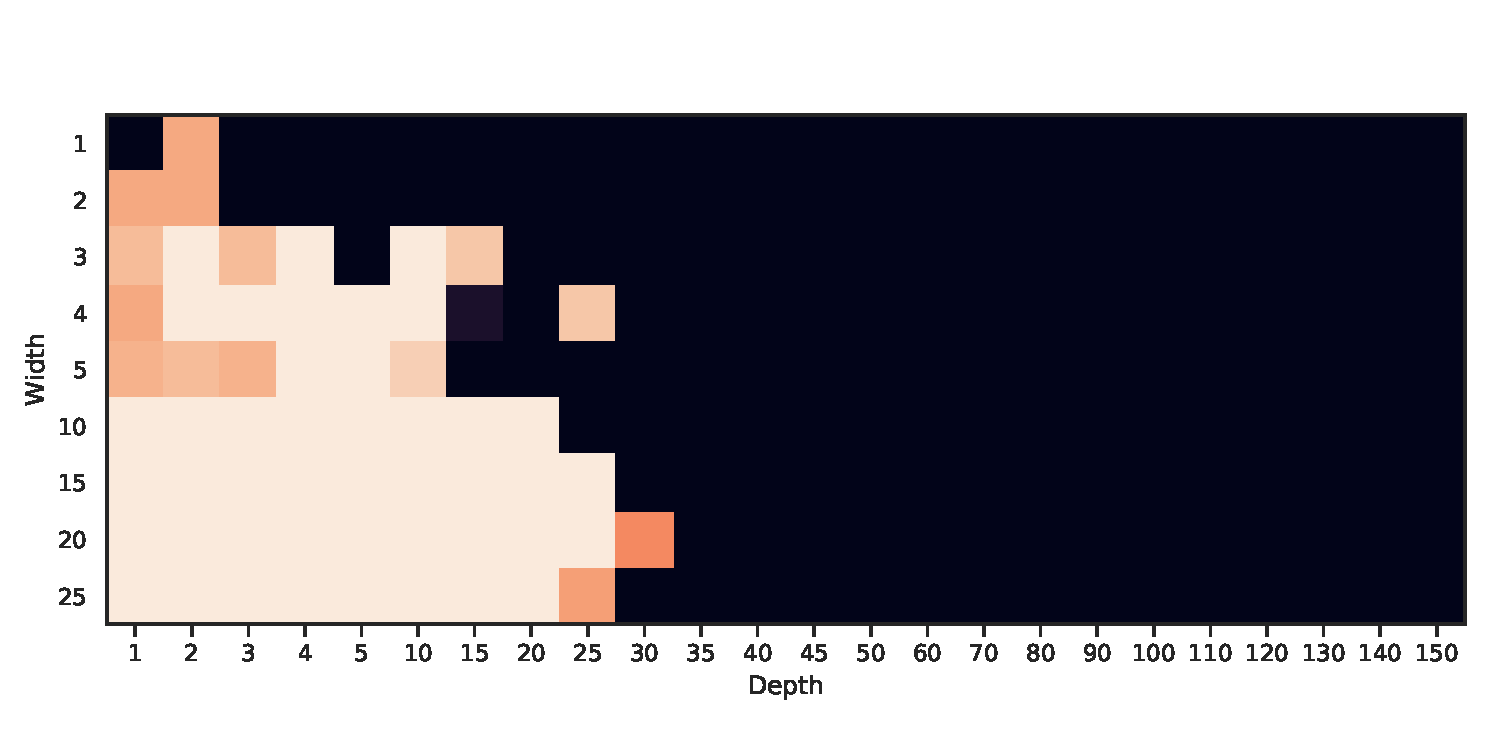
\includegraphics[width=\textwidth]{img/moons_grid/acc-relu.pdf}
        \caption{\ReLU training}
        \label{fig:moons_grid_relu}
    \end{subfigure}
    ~ %add desired spacing between images, e. g. ~, \quad, \qquad, \hfill etc. 
      %(or a blank line to force the subfigure onto a new line)
    \centering
    \begin{subfigure}[b]{0.3\textwidth}
        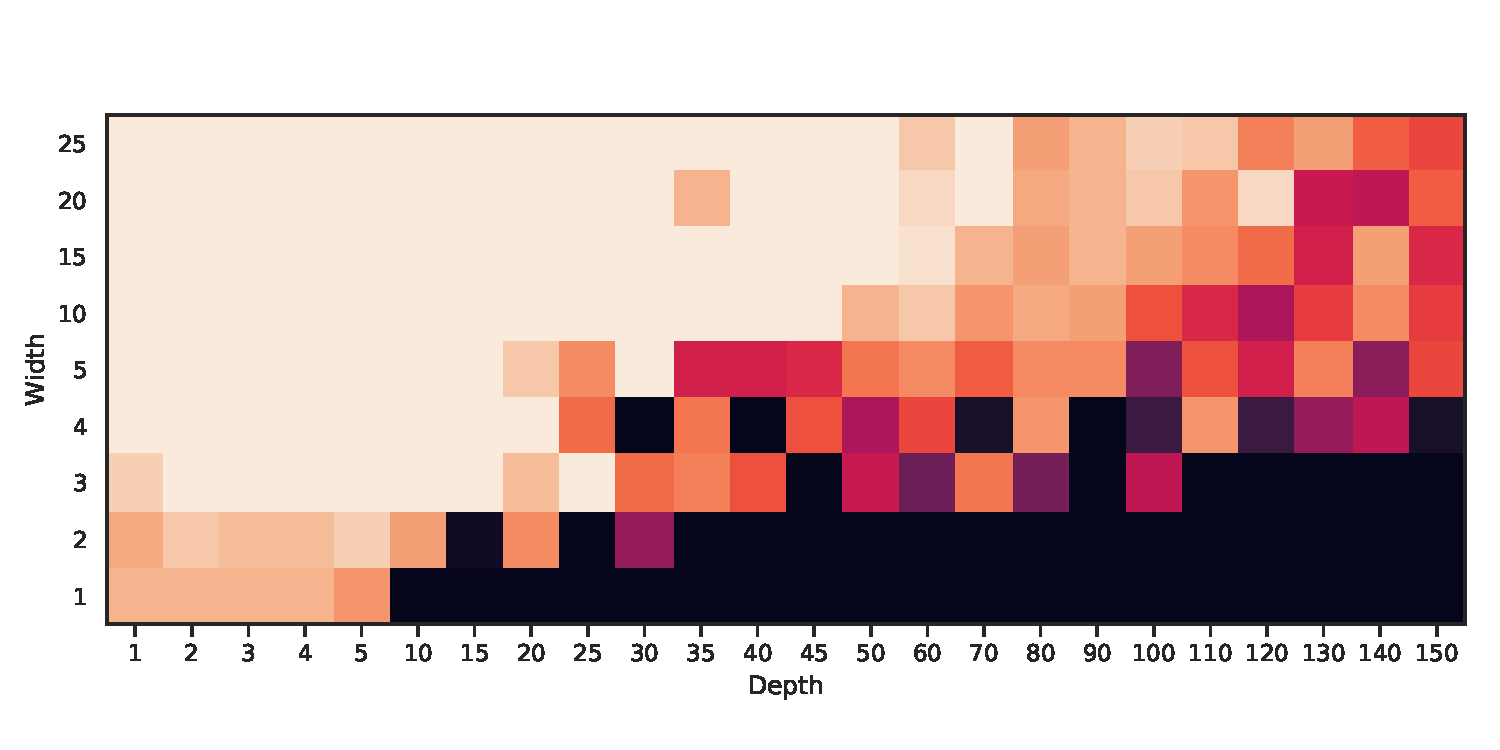
\includegraphics[width=\textwidth]{img/moons_grid/acc-relu-bn.pdf}
        \caption{\ReLUBN training}
        \label{fig:moons_grid_relubn}
    \end{subfigure}
    ~ %add desired spacing between images, e. g. ~, \quad, \qquad, \hfill etc. 
      %(or a blank line to force the subfigure onto a new line)
    \centering
    \begin{subfigure}[b]{0.3\textwidth}
        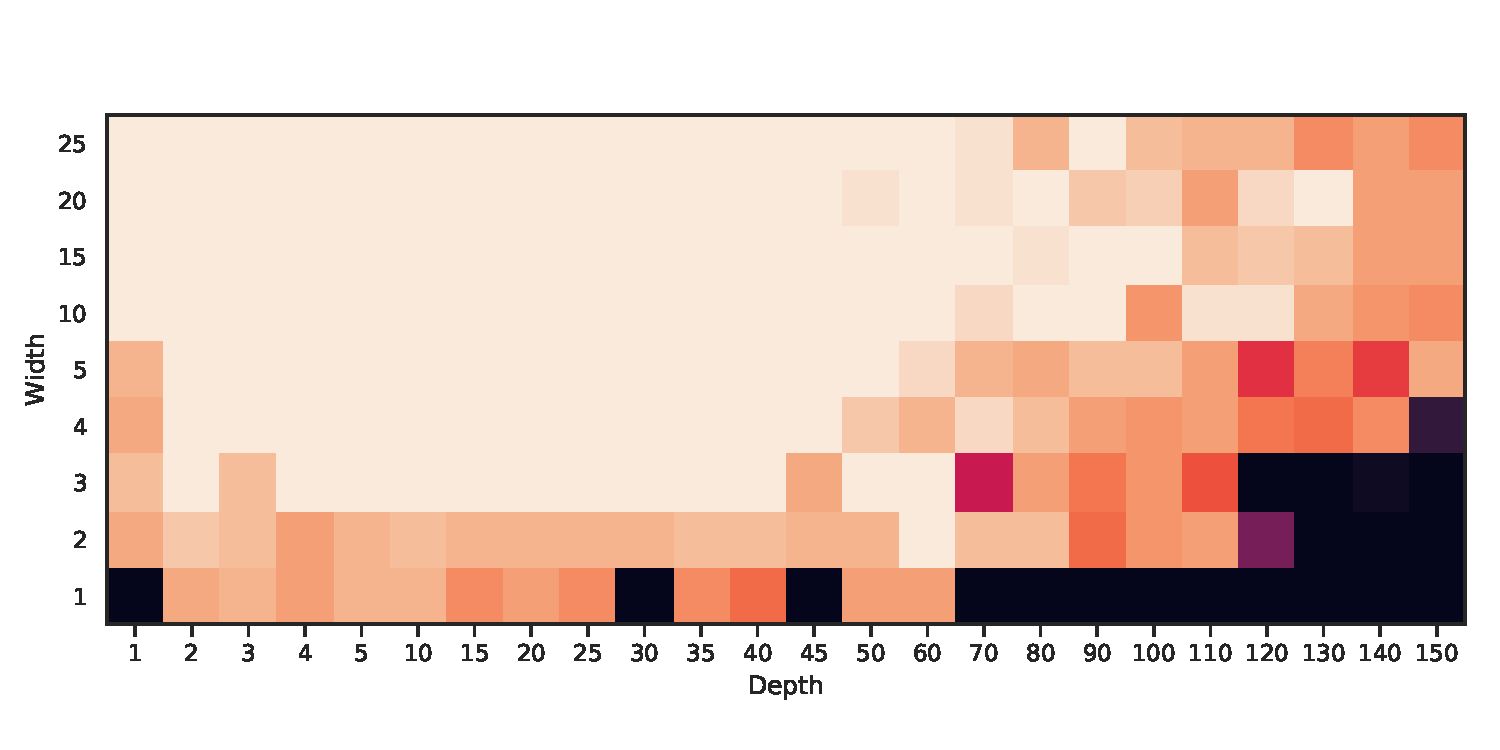
\includegraphics[width=\textwidth]{img/moons_grid/acc-sep-up-0-0001.pdf}
        \caption{\SepUnitPoint training}
        \label{fig:moons_grid_up}
    \end{subfigure}
    ~ %add desired spacing between images, e. g. ~, \quad, \qquad, \hfill etc. 
      %(or a blank line to force the subfigure onto a new line)
    \\
    \begin{subfigure}[b]{0.3\textwidth}
        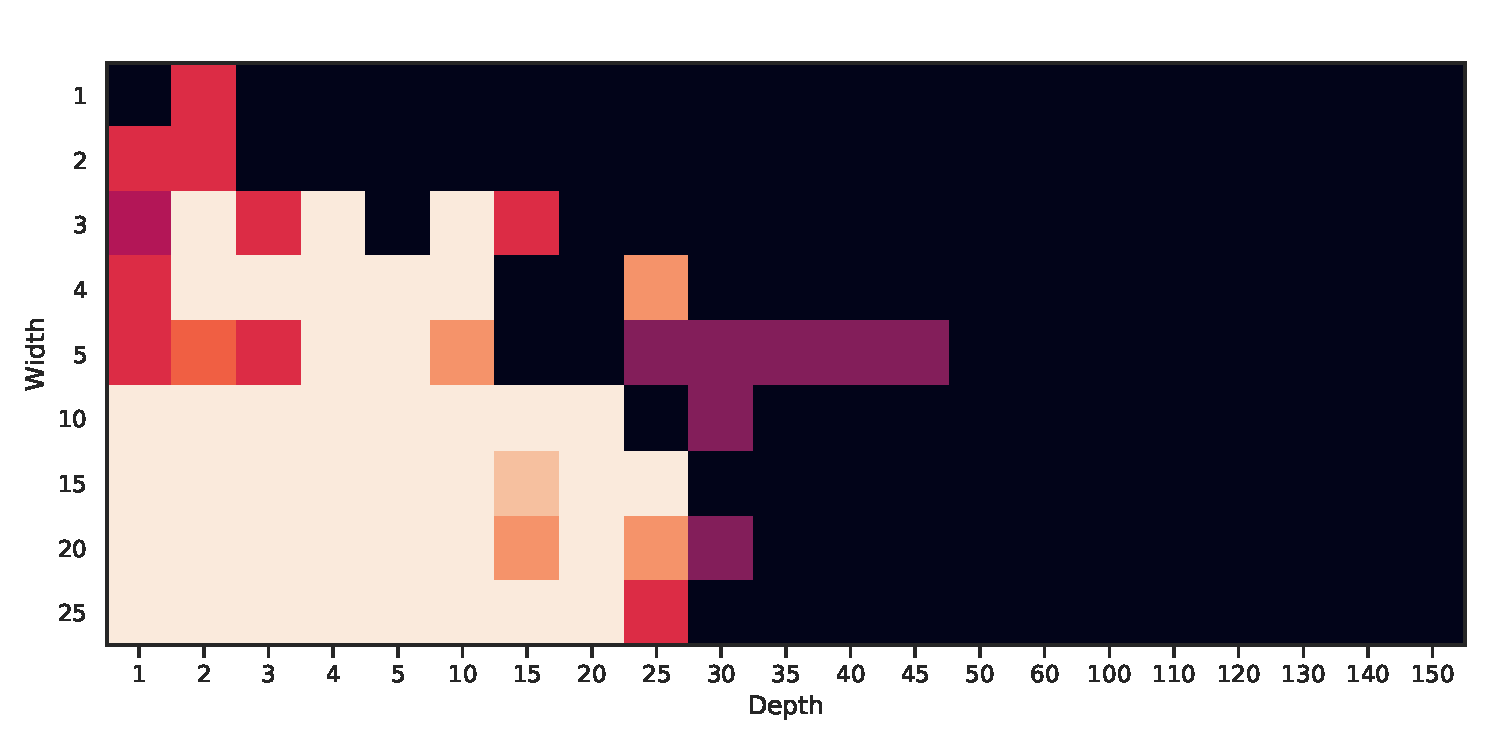
\includegraphics[width=\textwidth]{img/moons_grid/val-acc-relu.pdf}
        \caption{\ReLU validation}
        \label{fig:moons_grid_relu}
    \end{subfigure}
    ~ %add desired spacing between images, e. g. ~, \quad, \qquad, \hfill etc. 
      %(or a blank line to force the subfigure onto a new line)
    \centering
    \begin{subfigure}[b]{0.3\textwidth}
        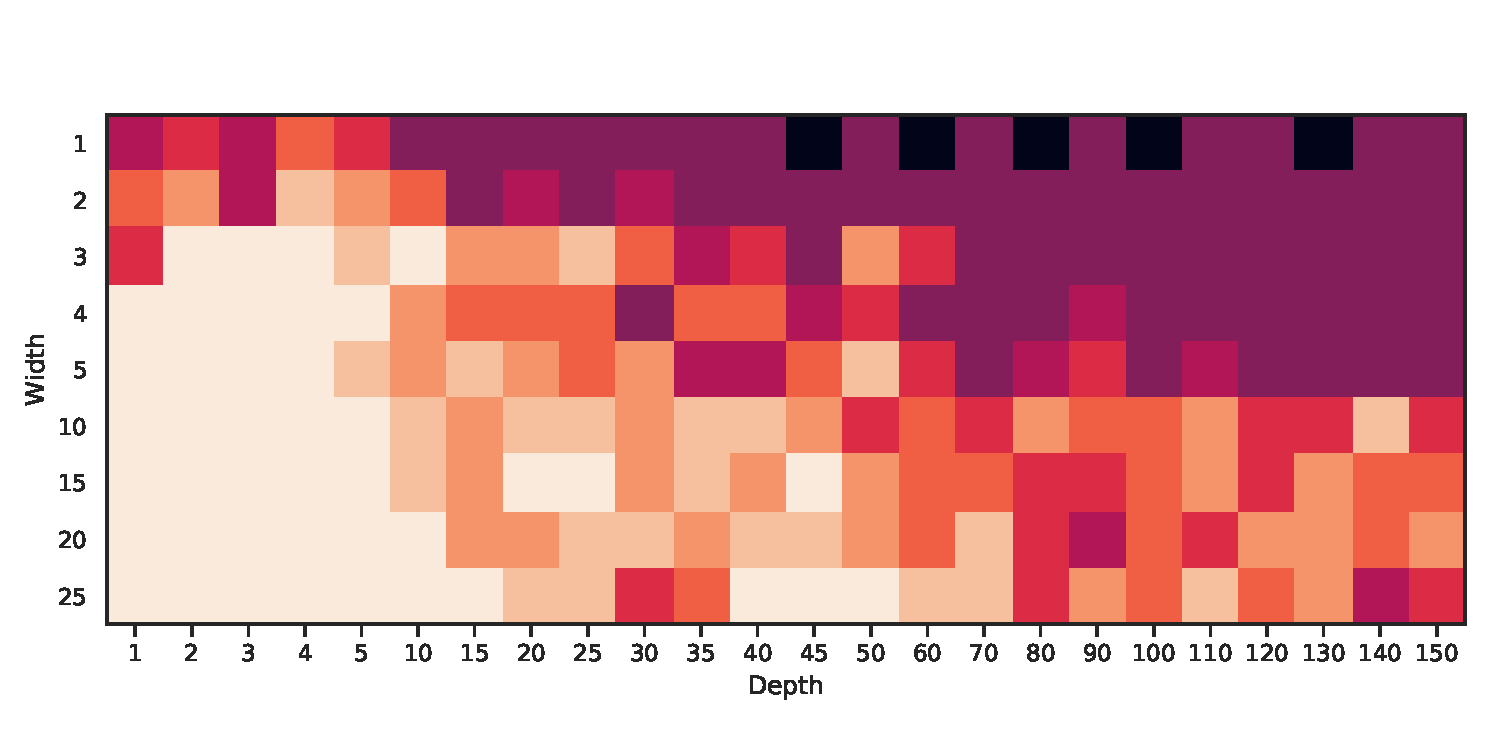
\includegraphics[width=\textwidth]{img/moons_grid/val-acc-relu-bn.pdf}
        \caption{\ReLUBN validation}
        \label{fig:moons_grid_relubn}
    \end{subfigure}
    ~ %add desired spacing between images, e. g. ~, \quad, \qquad, \hfill etc. 
      %(or a blank line to force the subfigure onto a new line)
    \centering
    \begin{subfigure}[b]{0.3\textwidth}
        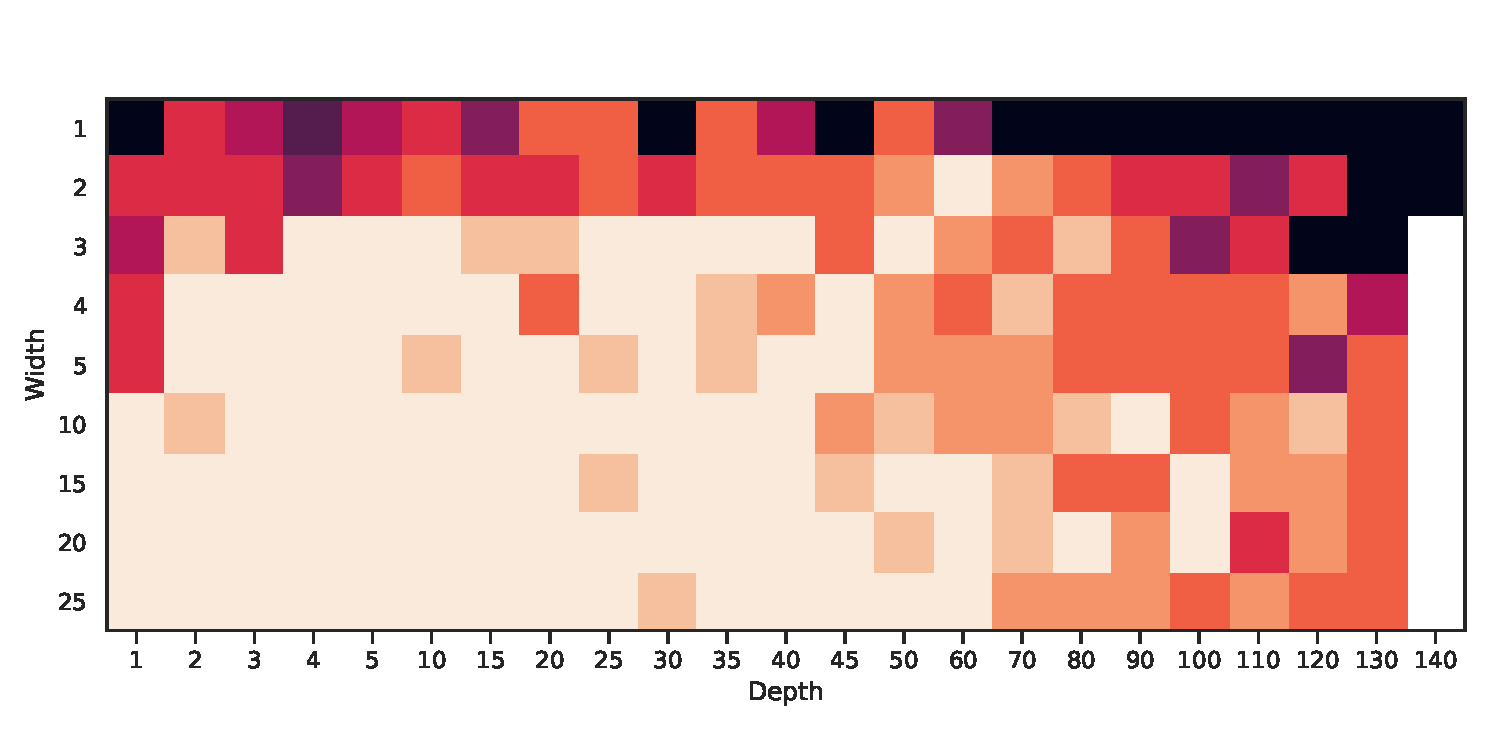
\includegraphics[width=\textwidth]{img/moons_grid/val-acc-sep-up-0-0001.pdf}
        \caption{\SepUnitPoint validation}
        \label{fig:moons_grid_up}
    \end{subfigure}
    ~ %add desired spacing between images, e. g. ~, \quad, \qquad, \hfill etc. 
      %(or a blank line to force the subfigure onto a new line)
      \\
    \begin{subfigure}[b]{0.3\textwidth}
        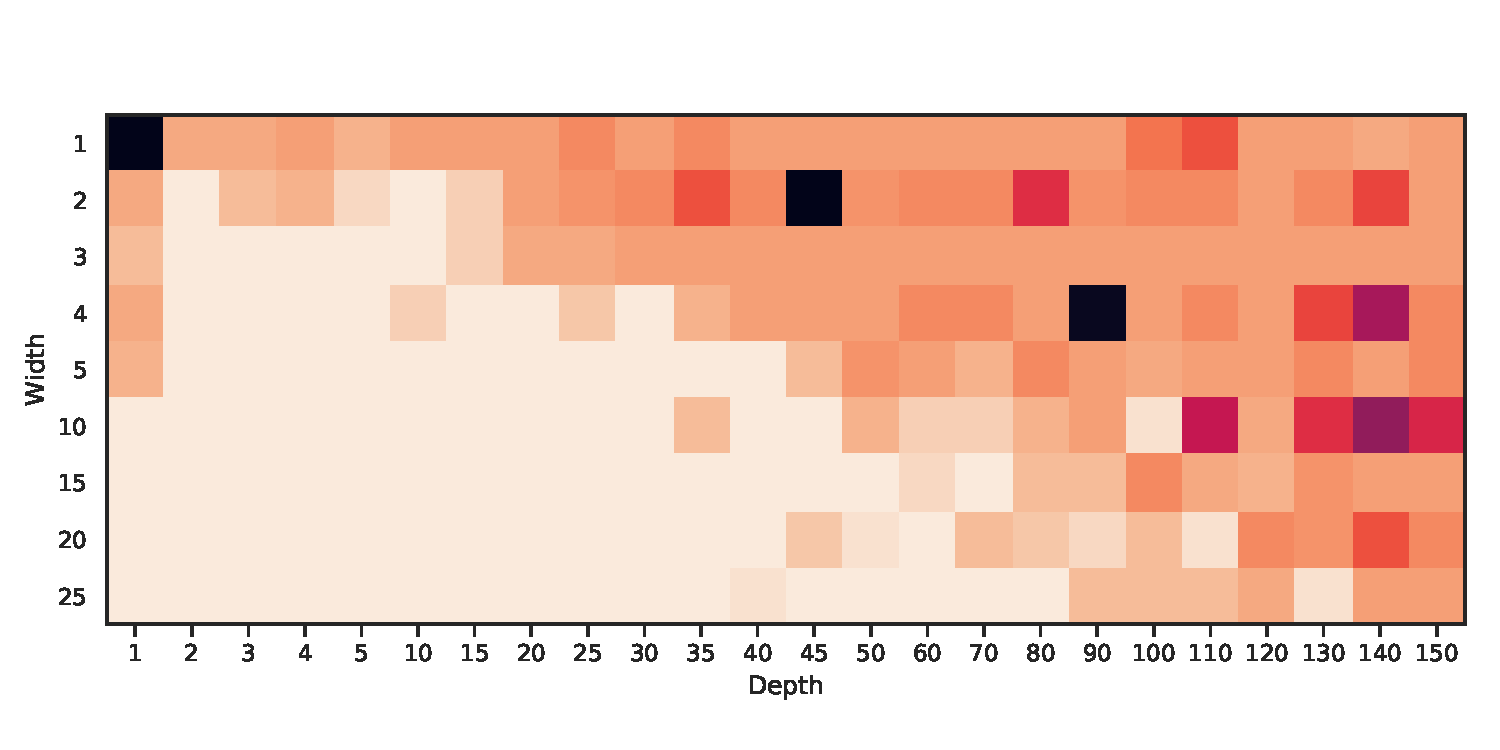
\includegraphics[width=\textwidth]{img/moons_grid/acc-sep-u-0-0001.pdf}
        \caption{\SepUnit training}
        \label{fig:moons_grid_u}
    \end{subfigure}
    ~ %add desired spacing between images, e. g. ~, \quad, \qquad, \hfill etc. 
      %(or a blank line to force the subfigure onto a new line)
    \centering
    \begin{subfigure}[b]{0.3\textwidth}
        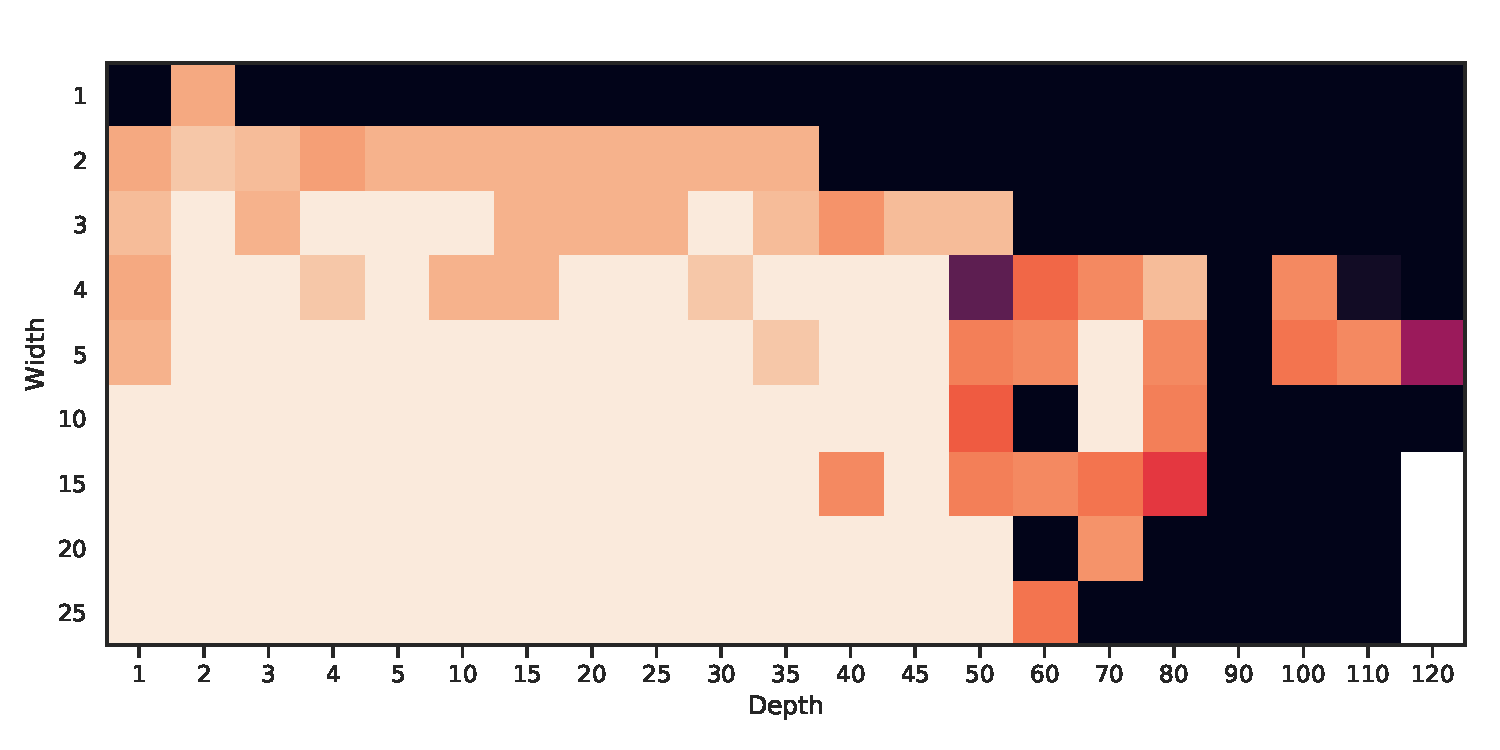
\includegraphics[width=\textwidth]{img/moons_grid/acc-sep-p-0-0001.pdf}
        \caption{\SepPoint training}
        \label{fig:moons_grid_p}
    \end{subfigure}
    ~ %add desired spacing between images, e. g. ~, \quad, \qquad, \hfill etc. 
      %(or a blank line to force the subfigure onto a new line)
    \\
    \begin{subfigure}[b]{0.3\textwidth}
        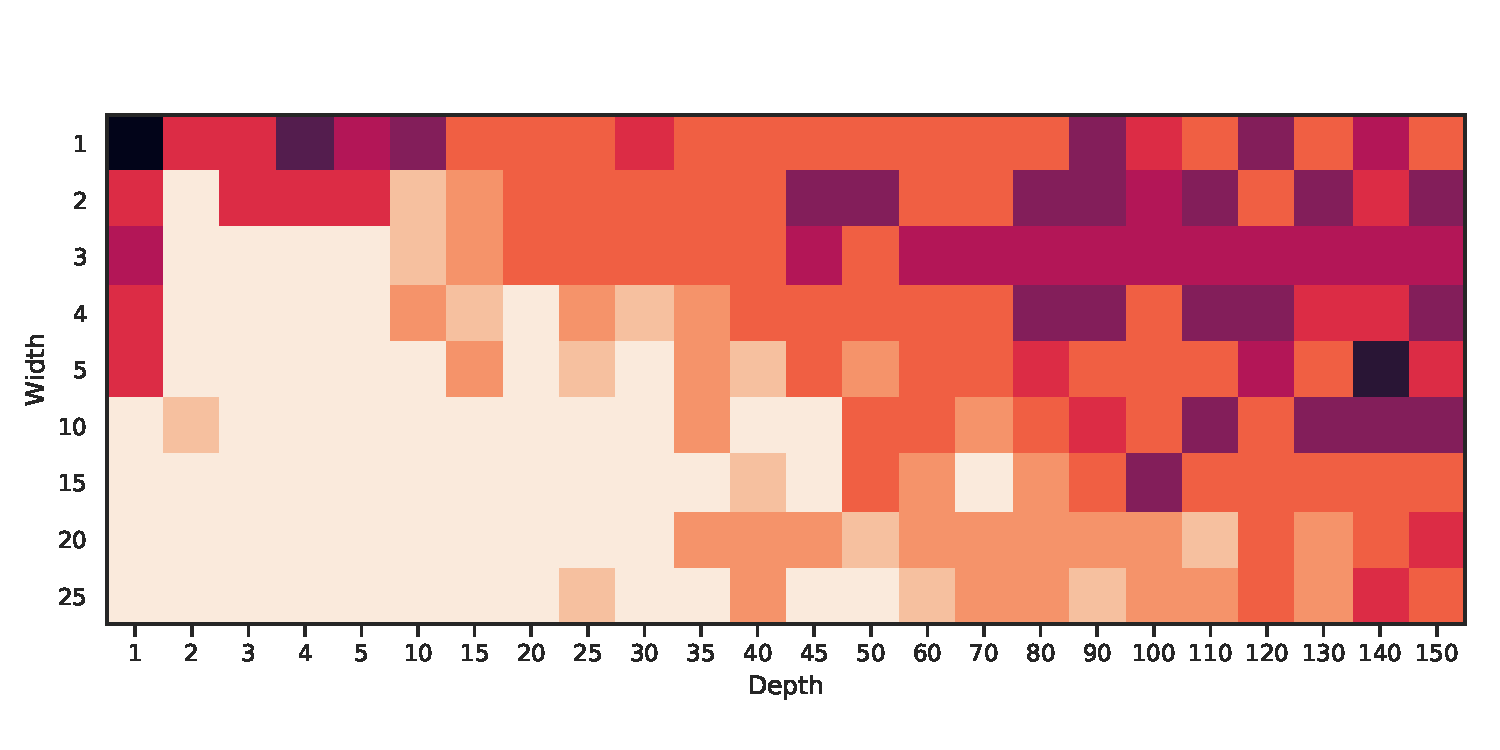
\includegraphics[width=\textwidth]{img/moons_grid/val-acc-sep-u-0-0001.pdf}
        \caption{\SepUnit validation}
        \label{fig:moons_grid_u}
    \end{subfigure}
    ~ %add desired spacing between images, e. g. ~, \quad, \qquad, \hfill etc. 
      %(or a blank line to force the subfigure onto a new line)
    \centering
    \begin{subfigure}[b]{0.3\textwidth}
        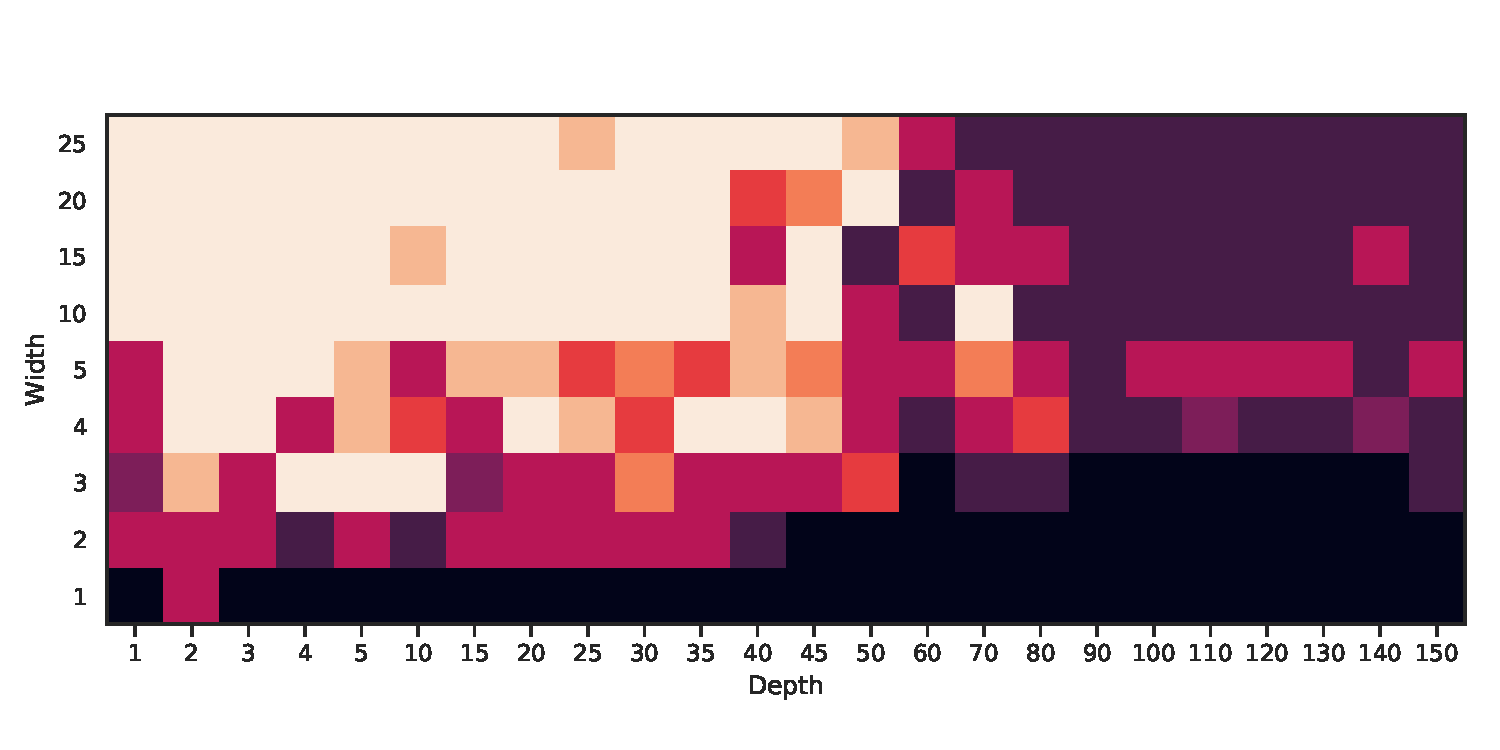
\includegraphics[width=\textwidth]{img/moons_grid/val-acc-sep-p-0-0001.pdf}
        \caption{\SepPoint validation}
        \label{fig:moons_grid_p}
    \end{subfigure}
    ~ %add desired spacing between images, e. g. ~, \quad, \qquad, \hfill etc. 
      %(or a blank line to force the subfigure onto a new line)
    
    
  \caption{Depth vs Width accuracy plot a for rectangular network using a grid (width from $2$ to $25$ and depth from $2$ to $150$),  trained using a Adam learning rate of $0.01$ in the \moons dataset. The color show the accuracy attained of each of the combinations of width and depth, the clearer the better. Notice how \ReLU, Figure \ref{fig:moons_grid_relu}, fails with networks deeper than 30 layers. In other hand, \ReLUBN, Figure \ref{fig:moons_grid_relubn}, manages to work until 70 layers deep. \SepUnitPoint,  Figure \ref{fig:moons_grid_up}, works significantly better than both, up to 120 layers. Notice how all the methods suffer from degradation from depth, which is partially alleviated by the use of greater width. This is consistent with \cite{simpnet} and \cite{densenet}. However, \SepUnitPoint is able to delay the apparition of the issue. This is especially visible when the number of units is small (from $2$ to $5$) where \ReLUBN fails to work whereas \SepUnitPoint does not. Regarding to the role of the constraint on its success, we find that \SepUnit, Figure \ref{fig:moons_grid_u}, allows the network to grow deeper, yet the accuracy can be lower following the linear decrease with the inverse of the width, which we blame on the inability of the \SepUnit constraint to address the \emph{dead point} issue. In the other hand, \SepPoint, Figure \ref{fig:moons_grid_p}, seems to perform well up to 50 layers, but it breaks down afterwards. Finally, \SepLayer , Figure \ref{fig:moons_grid_l} seems to suffer if the width is too large, performing well up to 70 layers.}
  \label{fig:moons_grid} 
\end{figure*}


\begin{figure*}
  \centering
    \begin{subfigure}[b]{0.3\textwidth}
        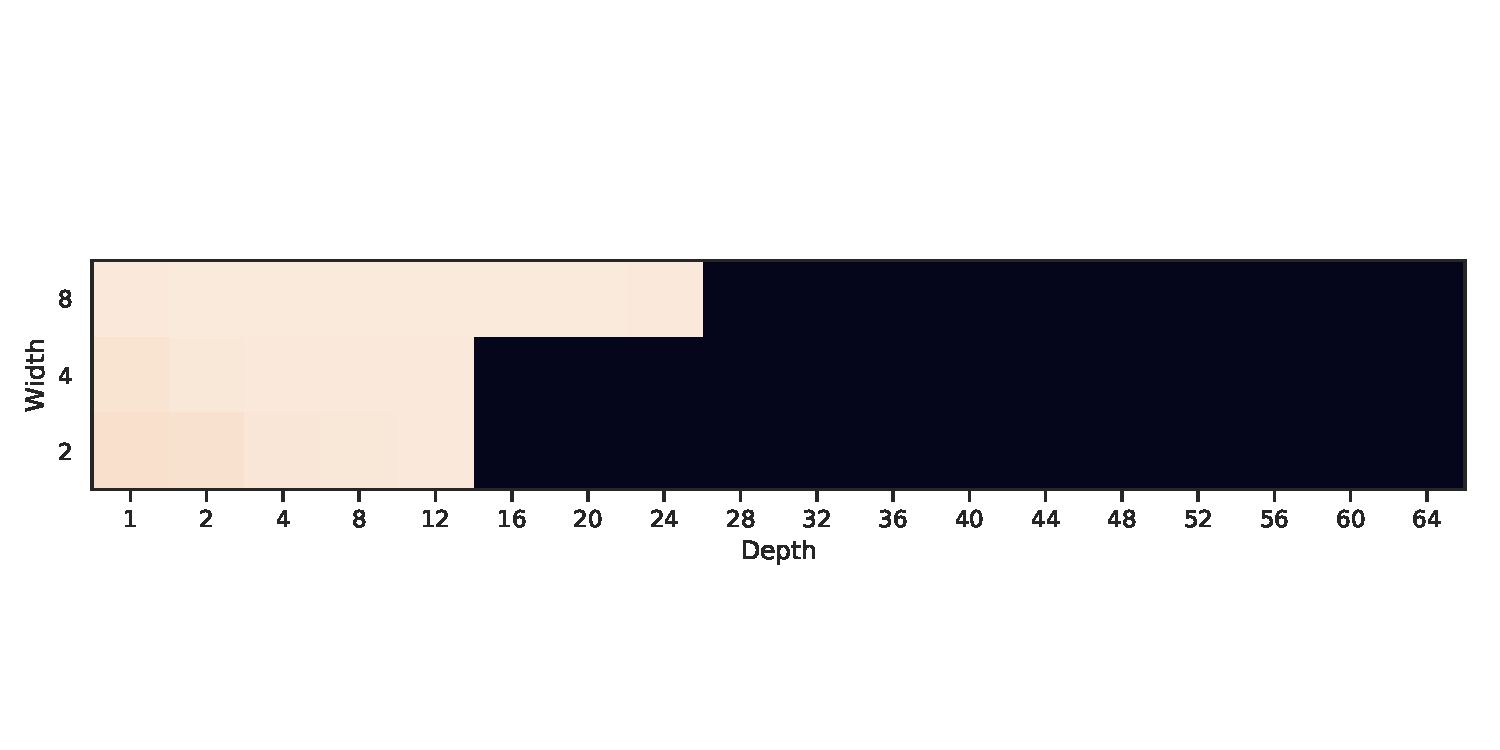
\includegraphics[width=\textwidth]{img/mnist_grid/acc-relu-ks-3x3-bs-1024.pdf}
        \caption{\ReLU}
        \label{fig:mnist_grid_relu}
    \end{subfigure}
    ~ %add desired spacing between images, e. g. ~, \quad, \qquad, \hfill etc. 
      %(or a blank line to force the subfigure onto a new line)
    \centering
    \begin{subfigure}[b]{0.3\textwidth}
        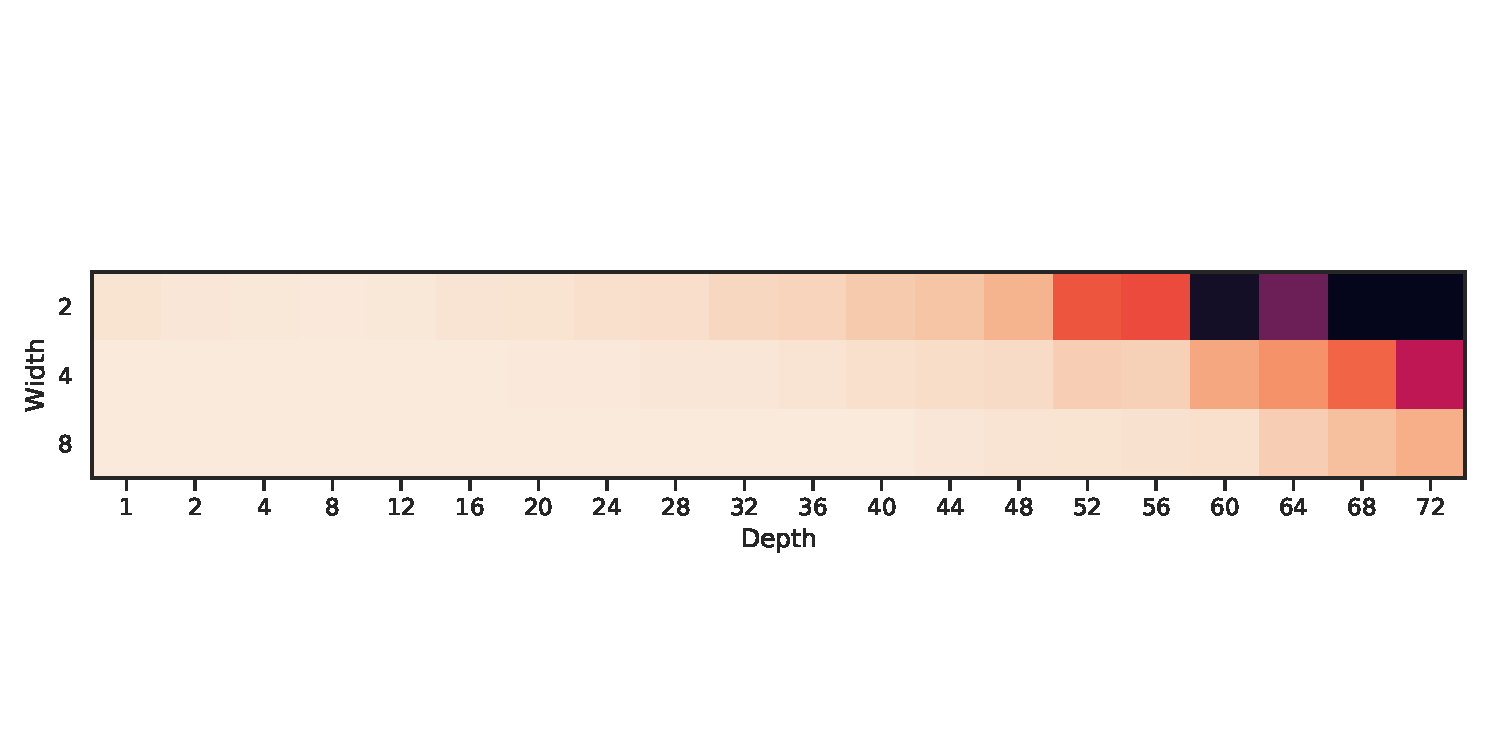
\includegraphics[width=\textwidth]{img/mnist_grid/acc-relu-bn-ks-3x3-bs-1024.pdf}
        \caption{\ReLUBN}
        \label{fig:mnist_grid_relubn}
    \end{subfigure}
    ~ %add desired spacing between images, e. g. ~, \quad, \qquad, \hfill etc. 
      %(or a blank line to force the subfigure onto a new line)
    \centering
    \begin{subfigure}[b]{0.3\textwidth}
        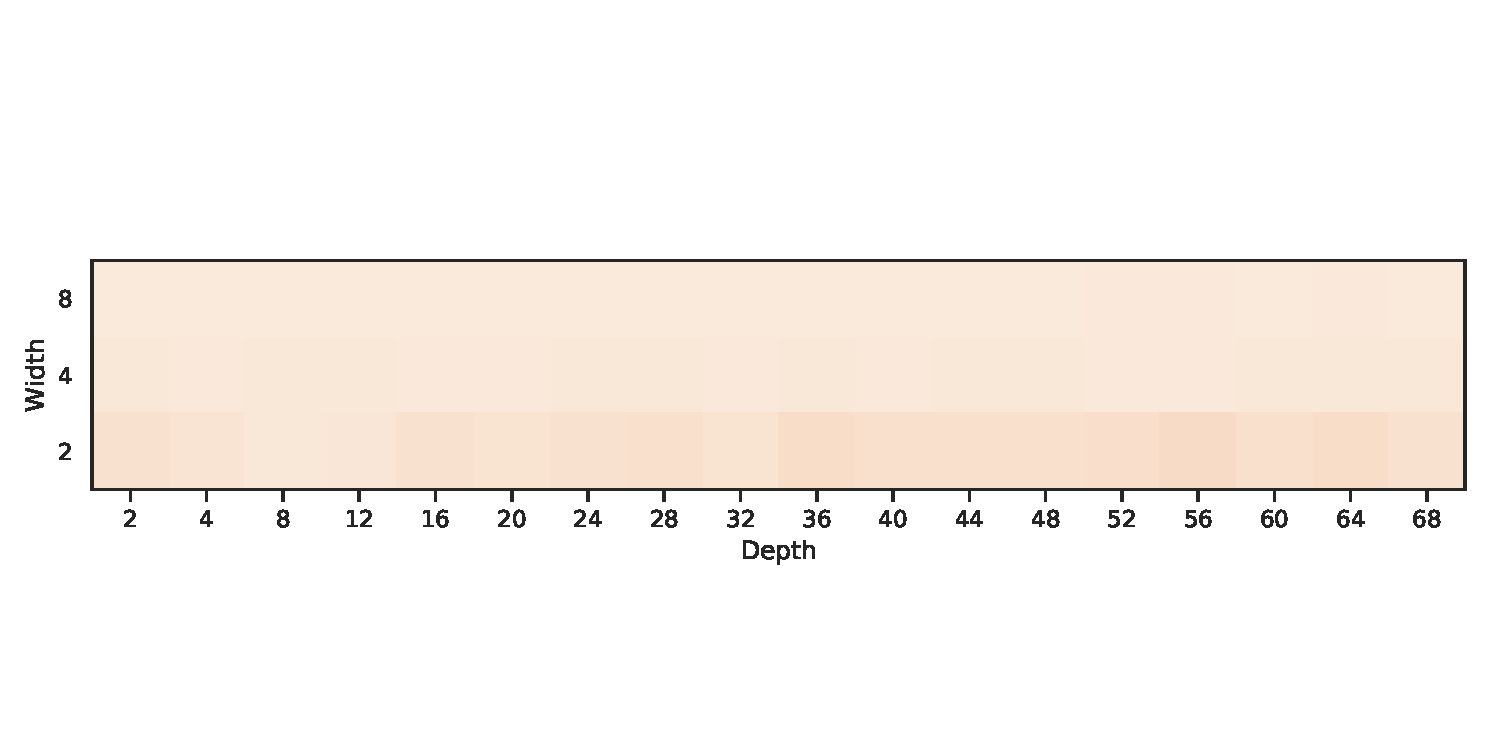
\includegraphics[width=\textwidth]{img/mnist_grid/acc-sep-up-1e-08-ks-3x3-bs-1024.pdf}
        \caption{\SepUnitPoint}
        \label{fig:mnist_grid_up}
    \end{subfigure}
    ~ %add desired spacing between images, e. g. ~, \quad, \qquad, \hfill etc. 
      %(or a blank line to force the subfigure onto a new line)
    
  \caption{Depth vs Width accuracy plot a for rectangular network using a grid (width from $2$ to $25$ and depth from $2$ to $150$),  trained using a Adam learning rate of $0.01$ in the MNIST dataset. The color show the accuracy attained of each of the combinations of width and depth, the clearer the better. Notice how \ReLU, Figure \ref{fig:mnist_grid_relu}, fails with networks deeper than 30 layers. In other hand, \ReLUBN, Figure \ref{fig:mnist_grid_relubn}, manages to work until 70 layers deep. \SepUnitPoint,  Figure \ref{fig:mnist_grid_up}, works significantly better than both, up to 120 layers. Notice how all the methods suffer from degradation from depth, which is partially alleviated by the use of greater width. This is consistent with \cite{simpnet} and \cite{densenet}. However, \SepUnitPoint is able to delay the apparition of the issue. This is especially visible when the number of units is small (from $2$ to $5$) where \ReLUBN fails to work whereas \SepUnitPoint does not.}
  \label{fig:mnist_grid} 
\end{figure*}



\begin{table*}
\begin{tabular}{llrrrrr}
\toprule
                    &    &       2  &       10 &       25 &       30 &       40 \\
\midrule
relu ks 3x3 & 10 &  0.72142 &  0.82748 &  0.09906 &  0.09880 &  0.09810 \\
relu-bn ks 3x3 & 10 &  0.90580 &  0.81764 &  0.70496 &  0.66718 &  0.59642 \\
Sep-UP 1e-08 ks 3x3 & 10 &  0.69264 &  0.79044 &  0.74344 &  0.70452 &  0.68416 \\
\bottomrule
\end{tabular}

\\
\begin{tabular}{llrrrrr}
\toprule
                    &    &      2  &      10 &      25 &      30 &      40 \\
\midrule
relu ks 3x3 & 10 &  0.5958 &  0.6052 &  0.1000 &  0.1000 &  0.1000 \\
relu-bn ks 3x3 & 10 &  0.5682 &  0.5385 &  0.5414 &  0.5328 &  0.4512 \\
Sep-UP 1e-08 ks 3x3 & 10 &  0.5874 &  0.5703 &  0.5353 &  0.5300 &  0.5320 \\
\bottomrule
\end{tabular}

\caption{}\label{tab:cifar10}
\end{table*}